\documentclass[UTF8,zihao=-4]{ctexart}
\usepackage[a4paper,margin=2.5cm]{geometry}
\usepackage{amsmath, amssymb, amsthm}
\usepackage{bm}
\usepackage{hyperref}
\usepackage{graphicx}
\usepackage{caption}
\usepackage{listings}
\usepackage{xcolor}
\usepackage{float}
\usepackage{placeins}
\graphicspath{{figures/}}

% Code style
\lstdefinestyle{code}{
  basicstyle=\ttfamily\small,
  numbers=left,
  numberstyle=\tiny,
  numbersep=8pt,
  keywordstyle=\color{blue},
  commentstyle=\color{teal!70!black},
  stringstyle=\color{orange!70!black},
  showstringspaces=false,
  breaklines=true,
  frame=single,
  framerule=0.3pt,
  rulecolor=\color{black!15}
}
\lstset{style=code}

\title{循环神经网络详解}
\author{}
\date{\today}

\begin{document}
\maketitle

\section{RNN 结构与原理}
循环神经网络(RNN)通过维护隐藏状态 $\mathbf{h}_t$ 对序列数据进行建模。基本 Elman RNN 的状态更新为
\begin{align}
  \mathbf{a}_t &= \mathbf{W}_{xh} \mathbf{x}_t + \mathbf{W}_{hh} \mathbf{h}_{t-1} + \mathbf{b}_h, \\
  \mathbf{h}_t &= \phi(\mathbf{a}_t), \\
  \mathbf{y}_t &= \mathbf{W}_{hy} \mathbf{h}_t + \mathbf{b}_y,
\end{align}
其中 $\phi$ 常取 $\tanh$ 或 ReLU。图~\ref{fig:rnn_unrolled_cn} 展示了将 RNN 在时间维展开后的计算图。

\subsection{展开与时间反向传播}
训练通过时间反向传播(BPTT)实现,将网络展开 $T$ 步并累加各时刻梯度:
\begin{equation}
  \frac{\partial \mathcal{L}}{\partial \mathbf{W}_{hh}} = \sum_{t=1}^{T} \left( \frac{\partial \mathcal{L}}{\partial \mathbf{a}_t} \frac{\partial \mathbf{a}_t}{\partial \mathbf{W}_{hh}} \right).
\end{equation}
多次相乘的递归权重可能导致梯度爆炸或消失,可通过梯度裁剪、正交初始化、残差连接等手段缓解。

\subsection{循环结构的拓展}
双向 RNN 同时沿前向与反向处理序列,拼接隐藏状态以利用上下文。堆叠(多层)RNN 构建层级表示;残差或 highway 连接有助于保持梯度。加入注意力或外部记忆可进一步增强长期依赖建模能力。

\begin{lstlisting}[language=Python, caption={PyTorch Elman RNN 单元示例。}]
import torch
import torch.nn as nn

class SimpleRNNCell(nn.Module):
    def __init__(self, input_size, hidden_size):
        super().__init__()
        self.Wxh = nn.Linear(input_size, hidden_size)
        self.Whh = nn.Linear(hidden_size, hidden_size)

    def forward(self, x_t, h_prev):
        a_t = self.Wxh(x_t) + self.Whh(h_prev)
        h_t = torch.tanh(a_t)
        return h_t
\end{lstlisting}

\begin{figure}[H]
  \centering
  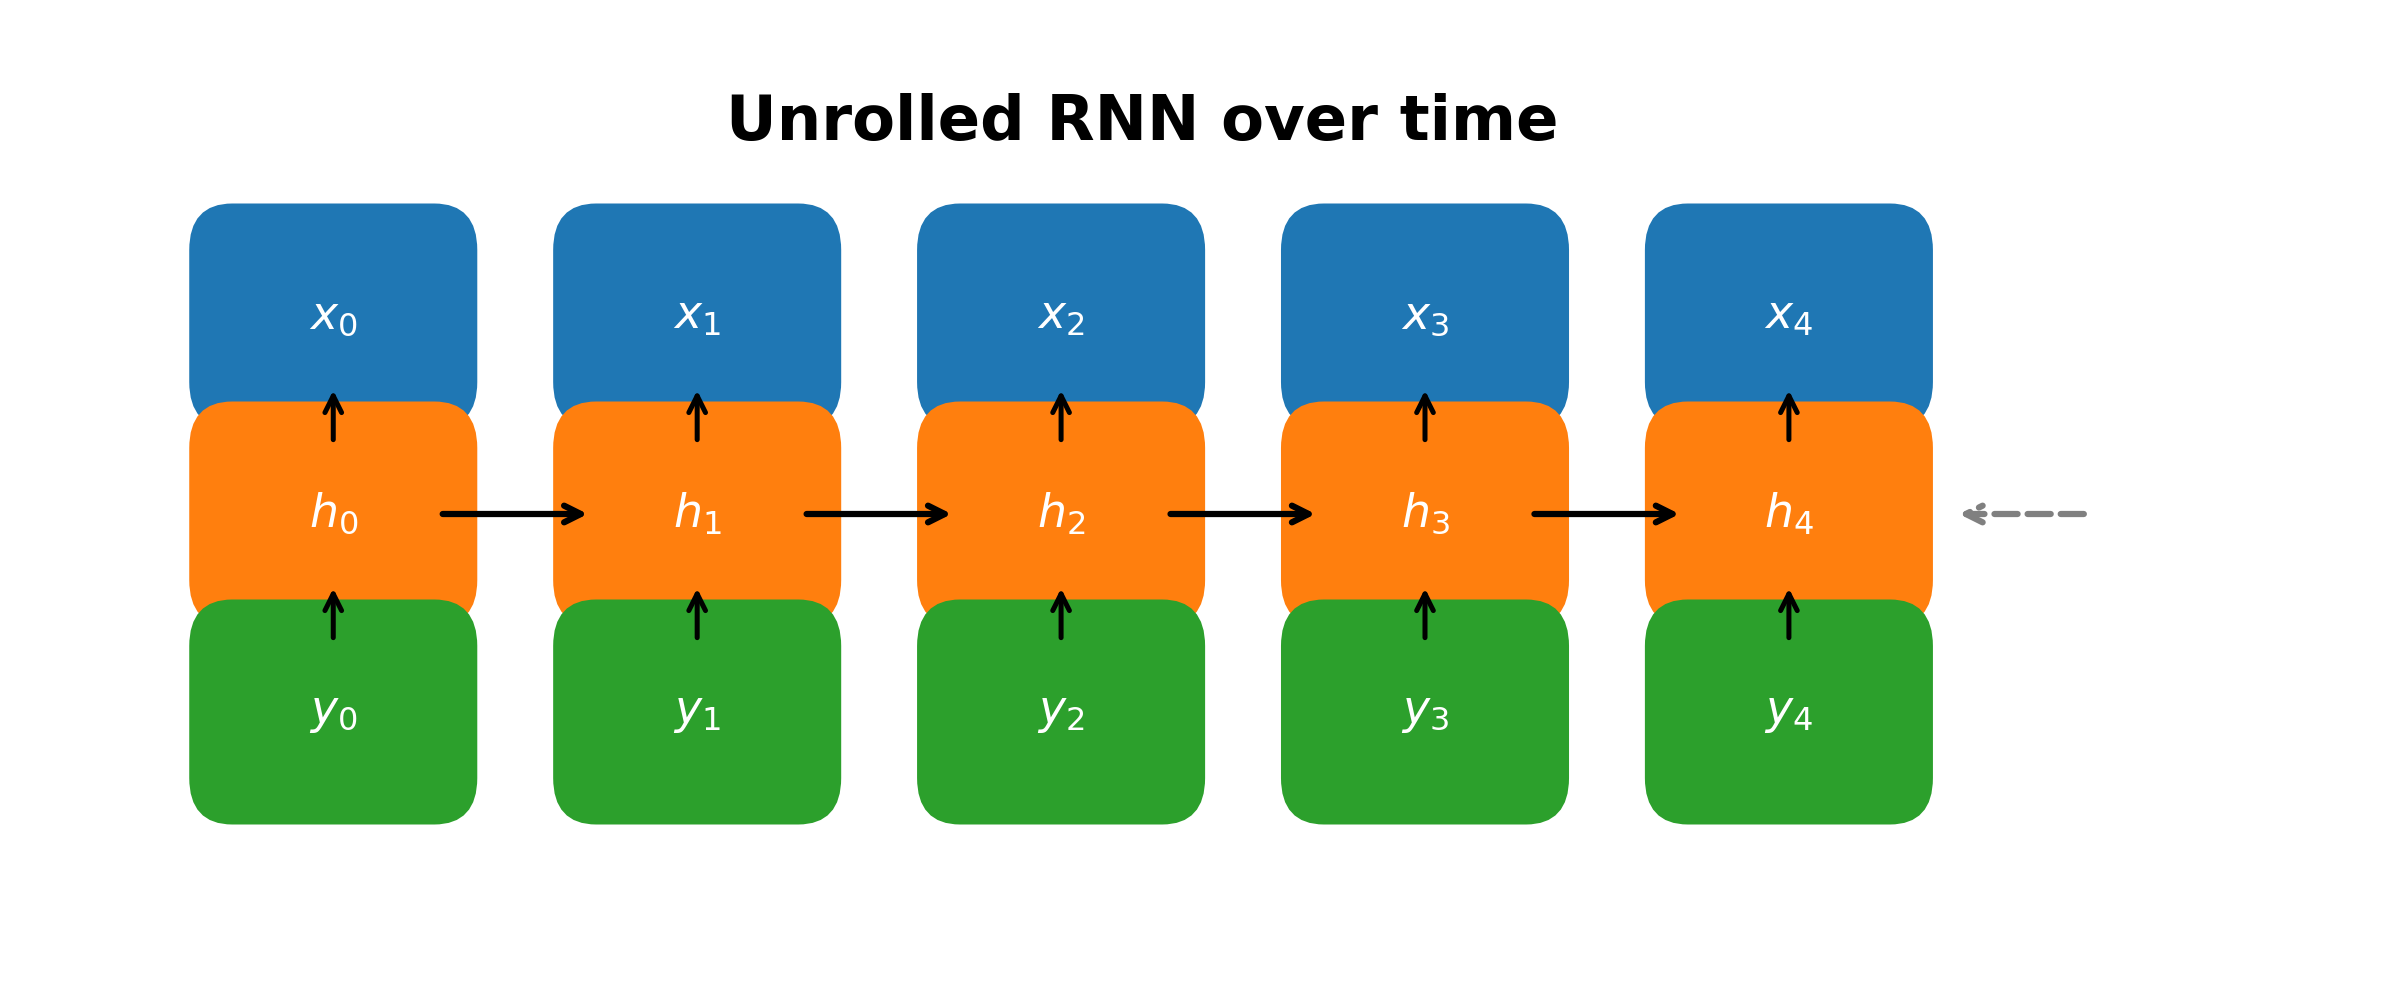
\includegraphics[width=0.85\linewidth]{rnn_unrolled_dynamics.png}
  \caption{RNN 在时间维展开后的信息流示意。}
  \label{fig:rnn_unrolled_cn}
\end{figure}
\FloatBarrier

\section{LSTM 与 GRU 的结构与原理}
长短时记忆网络(LSTM)与门控循环单元(GRU)利用门控机制缓解梯度消失并捕捉长程依赖。图~\ref{fig:lstm_gru_cn} 对比了两者的门控结构。

\subsection{LSTM 结构}
LSTM 维护细胞状态 $\mathbf{c}_t$ 与隐藏状态 $\mathbf{h}_t$:
\begin{align}
  \mathbf{f}_t &= \sigma(\mathbf{W}_f [\mathbf{x}_t, \mathbf{h}_{t-1}] + \mathbf{b}_f), \\
  \mathbf{i}_t &= \sigma(\mathbf{W}_i [\mathbf{x}_t, \mathbf{h}_{t-1}] + \mathbf{b}_i), \\
  \tilde{\mathbf{c}}_t &= \tanh(\mathbf{W}_c [\mathbf{x}_t, \mathbf{h}_{t-1}] + \mathbf{b}_c), \\
  \mathbf{c}_t &= \mathbf{f}_t \odot \mathbf{c}_{t-1} + \mathbf{i}_t \odot \tilde{\mathbf{c}}_t, \\
  \mathbf{o}_t &= \sigma(\mathbf{W}_o [\mathbf{x}_t, \mathbf{h}_{t-1}] + \mathbf{b}_o), \\
  \mathbf{h}_t &= \mathbf{o}_t \odot \tanh(\mathbf{c}_t).
\end{align}
遗忘门 $\mathbf{f}_t$ 用于保留长期记忆,输入门与输出门分别控制细胞状态的更新与暴露。

\subsection{GRU 结构}
GRU 将细胞状态与隐藏状态合并,通过更新门与重置门调节信息:
\begin{align}
  \mathbf{z}_t &= \sigma(\mathbf{W}_z [\mathbf{x}_t, \mathbf{h}_{t-1}] + \mathbf{b}_z), \\
  \mathbf{r}_t &= \sigma(\mathbf{W}_r [\mathbf{x}_t, \mathbf{h}_{t-1}] + \mathbf{b}_r), \\
  \tilde{\mathbf{h}}_t &= \tanh(\mathbf{W}_h [\mathbf{x}_t, \mathbf{r}_t \odot \mathbf{h}_{t-1}] + \mathbf{b}_h), \\
  \mathbf{h}_t &= (1 - \mathbf{z}_t) \odot \mathbf{h}_{t-1} + \mathbf{z}_t \odot \tilde{\mathbf{h}}_t.
\end{align}
GRU 参数更少、收敛更快,同时仍能建模长短期依赖。

\subsection{门控机制分析}
LSTM 与 GRU 依靠 Sigmoid 门对历史信息加权。可选的窥视孔(peephole)连接使门直接感知细胞状态。门内的层归一化有助稳定长序列训练。

\begin{figure}[H]
  \centering
  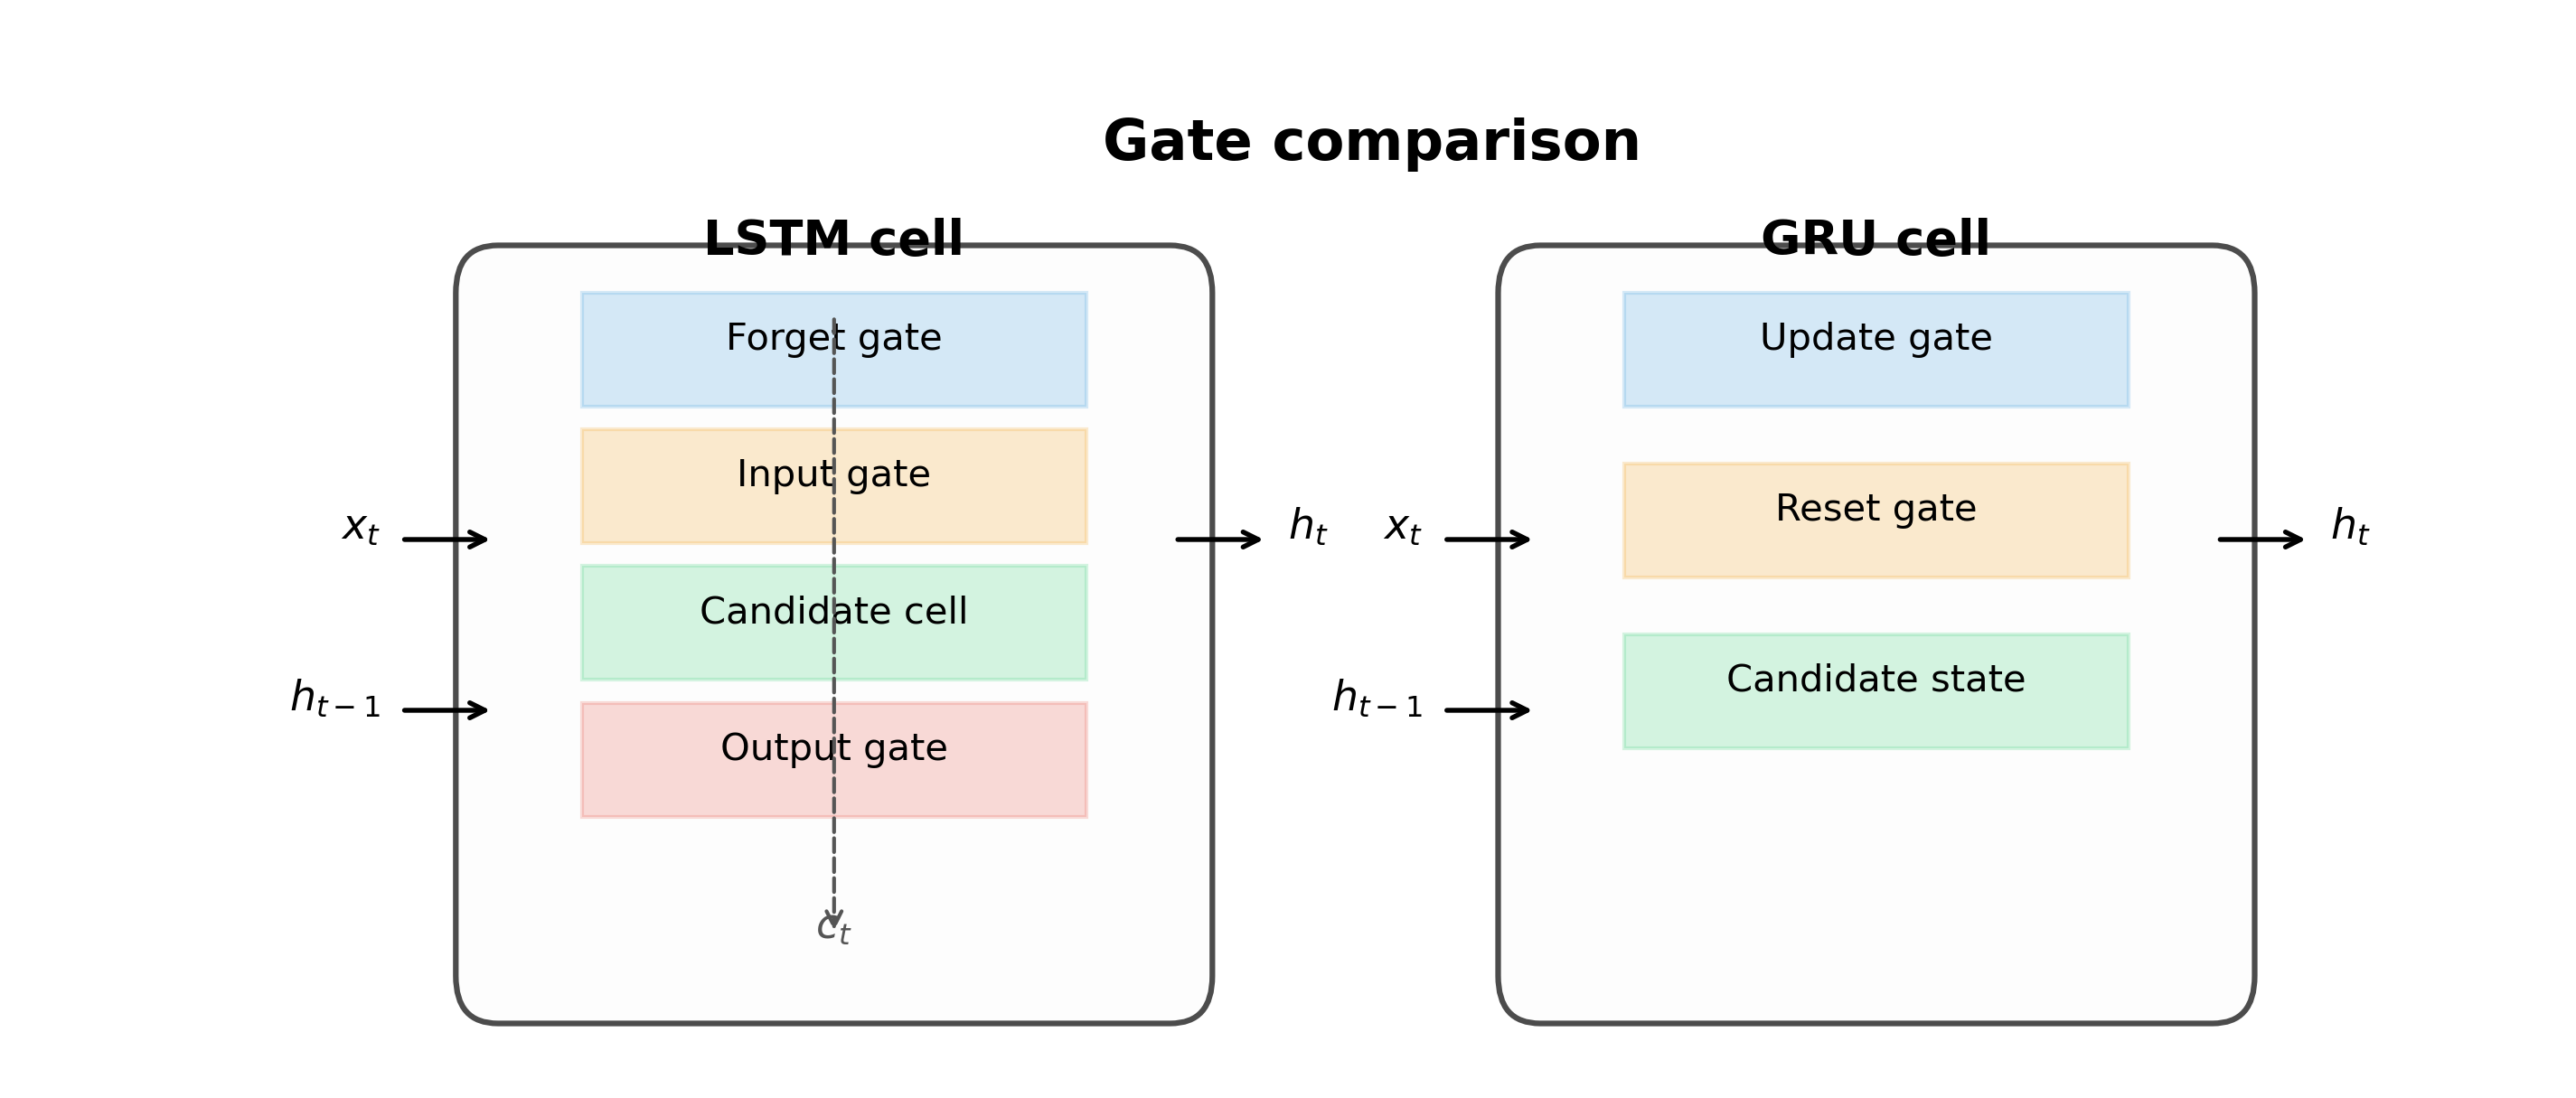
\includegraphics[width=0.85\linewidth]{lstm_gru_gate_comparison.png}
  \caption{LSTM 与 GRU 门控结构的信息流对比。}
  \label{fig:lstm_gru_cn}
\end{figure}
\FloatBarrier

\section{应用:时间序列预测、文本生成、语音建模}
RNN 广泛应用于序列数据建模。图~\ref{fig:rnn_applications_cn} 概括了三类典型应用流程。

\subsection{时间序列预测}
在预测任务中,RNN 接收历史观测值输出未来序列。编码器-解码器结构结合注意力可捕捉长距离依赖;采用高斯混合或分位数损失可量化预测不确定性。

\subsection{文本生成与语言建模}
字符级或词级 RNN 建模条件分布 $p(w_t \mid w_{<t})$。Teacher forcing 与 scheduled sampling 控制训练与推理的一致性;温度采样、top-k/top-p 策略影响生成多样性。结合词向量或子词表示能提升语义表达。

\subsection{语音与音频建模}
RNN 可处理可变长的声学序列。CTC 损失无需对齐即可训练语音识别模型;在语音合成中,WaveRNN 等自回归声码器逐样生成波形。多任务训练(声学 + 语言模型)提高识别准确率。

\subsection{混合架构}
注意力机制与 Transformer 在 RNN 基础上进一步增强长程依赖建模。神经常微分方程、连续时间 RNN 适用于非均匀采样数据;轻量门控单元(SRU、QRNN)减少串行依赖,提高推理速度。

\begin{figure}[H]
  \centering
  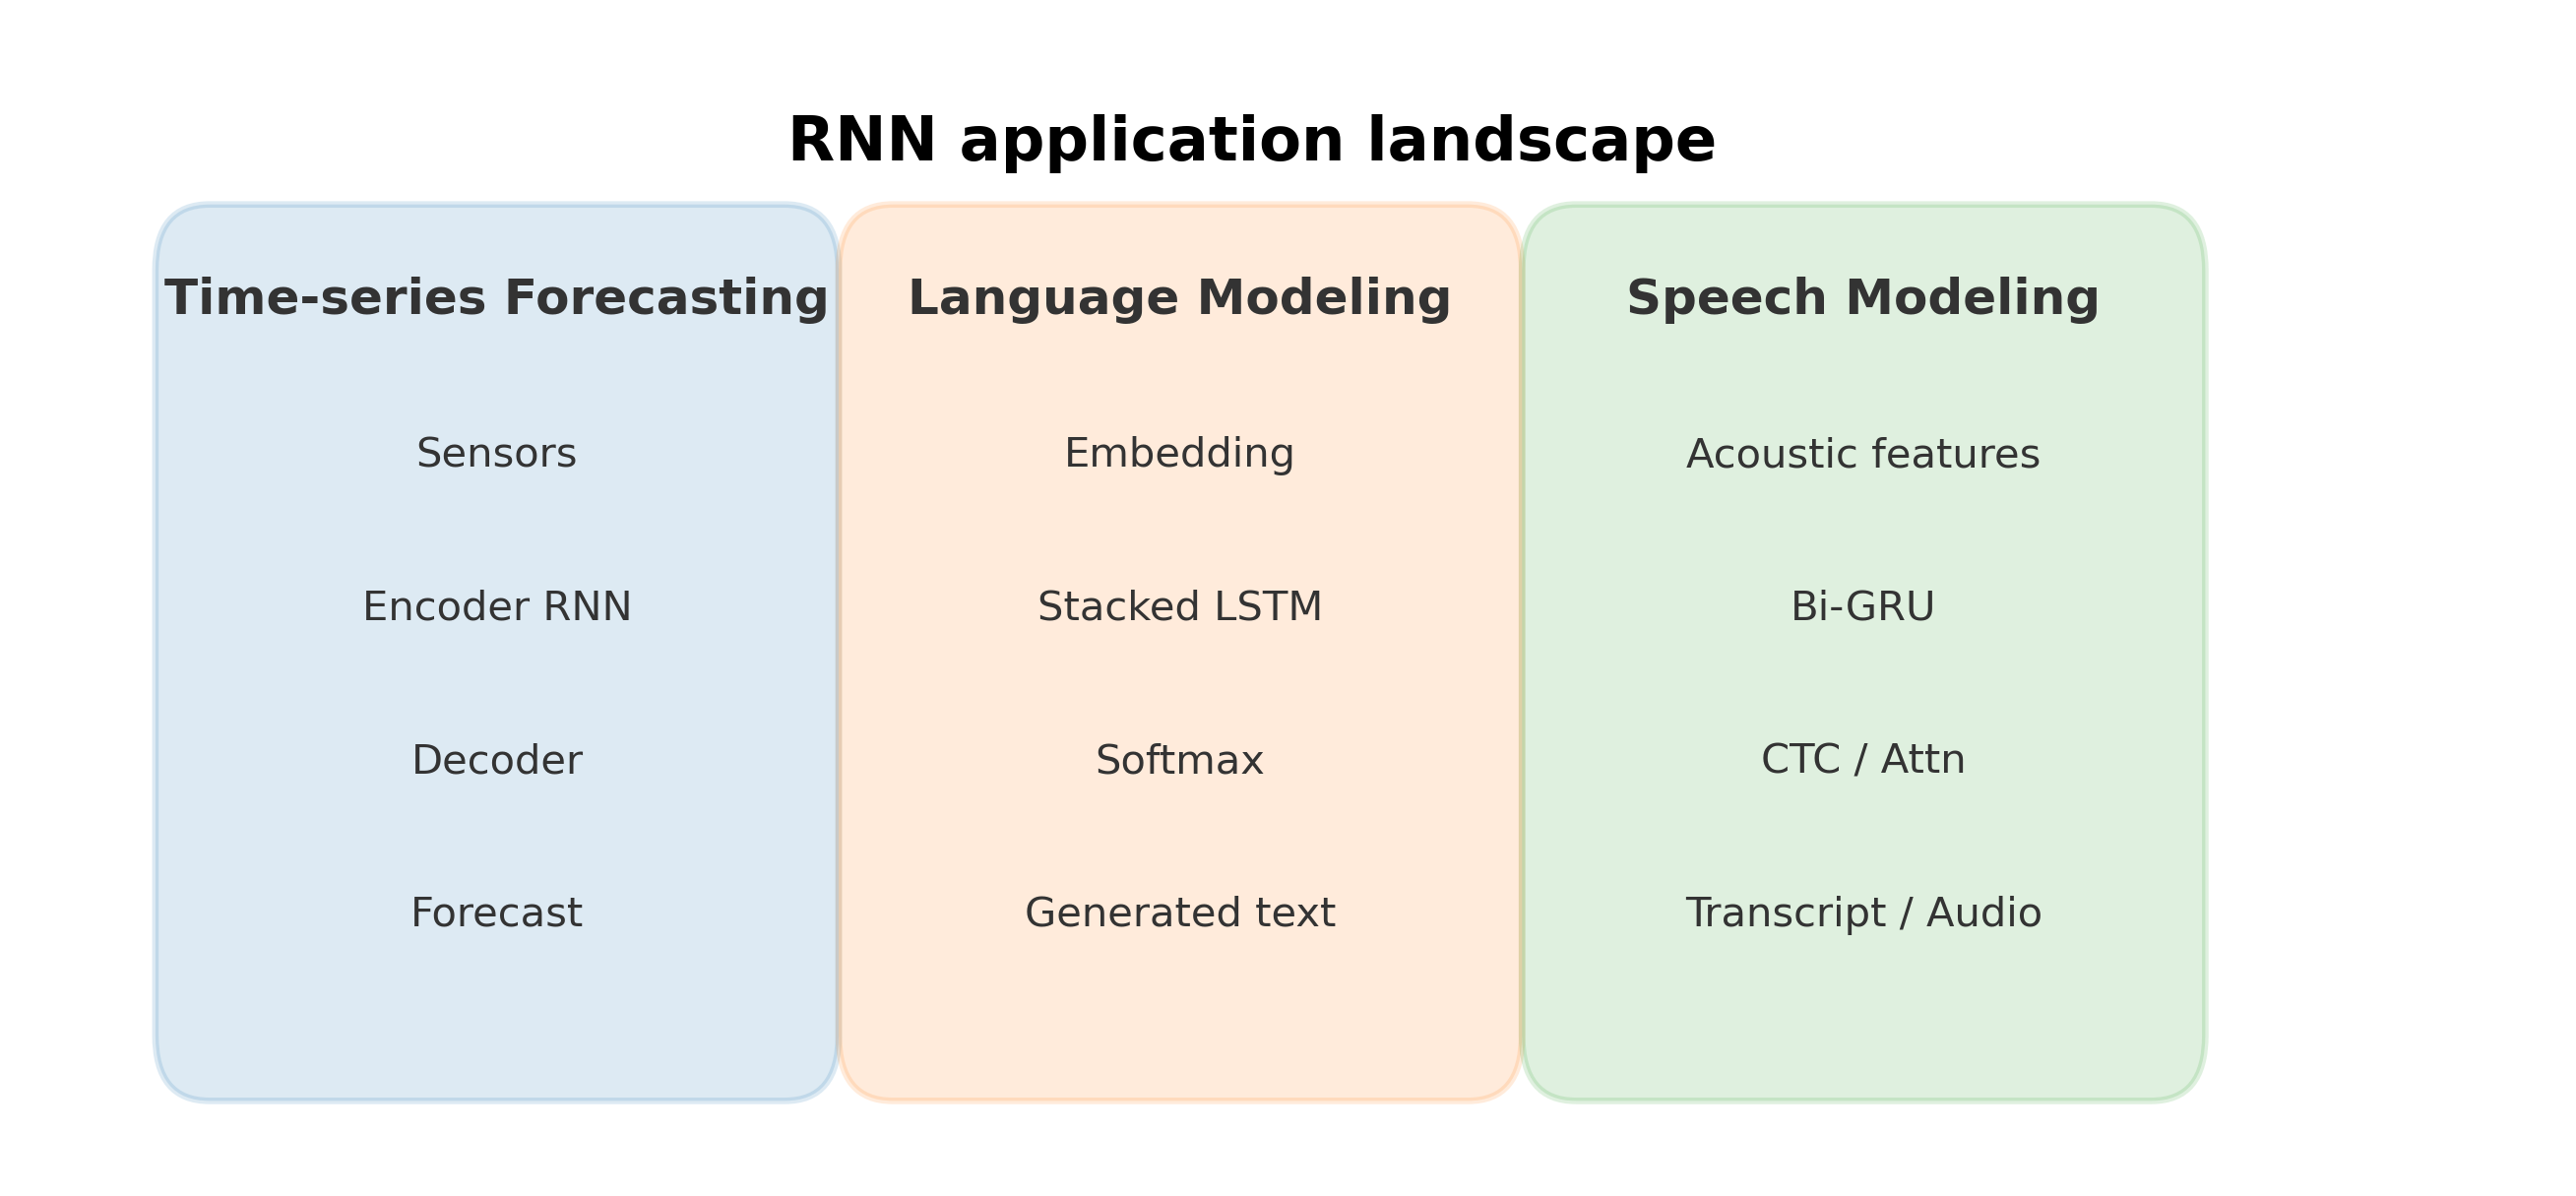
\includegraphics[width=0.85\linewidth]{rnn_applications_overview.png}
  \caption{RNN 在预测、语言建模、语音处理中的应用流程。}
  \label{fig:rnn_applications_cn}
\end{figure}
\FloatBarrier

\section{实践建议}
\begin{itemize}
  \item \textbf{序列长度:} 截断 BPTT 在计算成本与上下文范围间取得平衡。\item \textbf{正则化:} 输入 dropout、循环 dropout(变分 dropout)与权重衰减可防止过拟合。\item \textbf{初始化:} 对循环权重采用正交初始化有助保持梯度范数。\item \textbf{优化:} 结合动量 SGD 或 Adam 与全局范数裁剪提升训练稳定性。\item \textbf{监控指标:} 语言模型关注困惑度(Perplexity),预测任务关注 MAE/MAPE,语音识别关注字符或词错误率。\end{itemize}

\end{document}
